%
% resultat.tex 
%
% 
%
% !TEX root = ../../buch.tex
% !TEX encoding = UTF-8
%

\section{Resultat\label{antennen:resultat}}

Das Verfahren nach Ritz hat ergeben, dass die Antenne eine kreisförmige Abrundung aufweist. Es muss noch bestimmt werden, wie gross der Radius dieser Abrundungen ist. Hierfür kann wiederum das Verhältnis REF verwendet werden. Die Länge l, hierbei der Umfang des abgerundeten Dreiecks, sowie dessen Fläche A kann mit den Formeln
\begin{equation}
	l=2\cdot{\pi}\cdot{r}+3\cdot{s}-6\cdot{\sqrt{3}}\cdot{r}
	\label{antennen:Länge}
\end{equation}
\begin{equation}
	A=r^2\cdot{\pi}+3\cdot{r}\cdot{(s-2\cdot{\sqrt{3}}\cdot{r})}+\frac{\sqrt{3}\cdot{(s-2\cdot{\sqrt{3}}\cdot{r})^2}}{4}
	\label{antennen:Fläche}
\end{equation}
berechnet werden.
Der Wirkungsgrad ist nun zu einem Problem geworden, welches nur noch abhängig von der Seitenlänge s des Dreiecks und des Radius r der Kreise ist. Bildlich ist dies in Abbildung \ref{antennen:tikzdreieckAufteilung} veranschaulicht.
%TODO Erklären der Formeln l und A mittels Grafik (Formelabschnitte einfärben??)
\begin{figure}[htpb]
	\centering
	\begin{tikzpicture}
		% Define the length of the sides of the triangles
		\def\sidelength{3.14}
		
		% Calculate the height of the equilateral triangle
		\pgfmathsetmacro{\triangleheight}{sqrt(3)/2*\sidelength}
		% Draw the large outer triangle (white background)
		\draw[fill=white] (0,0) -- (\sidelength,0) -- (0.5*\sidelength, \triangleheight) -- cycle;
		\coordinate (A) at (0,0);
		\coordinate (B) at (2.51,0);
		\coordinate (C) at (2.51/2,1.73/2*2.51);
		% Verschiebung der Koordinaten um 10pt nach rechts und 10pt nach oben
		\coordinate (As) at ($(A) + (9pt,5pt)$);
		\coordinate (Bs) at ($(B) + (9pt,5pt)$);
		\coordinate (Cs) at ($(C) + (9pt,5pt)$);
		% Nodes with blue border and green fill
		\node[circle, inner sep=0pt, minimum size=9pt, fill=green, draw=blue, line width=1pt] at (As) {};
		\node[circle, inner sep=0pt, minimum size=9pt, fill=green, draw=blue, line width=1pt] at (Bs) {};
		\node[circle, inner sep=0pt, minimum size=9pt, fill=green, draw=blue, line width=1pt] at (Cs) {};
		
		% Black lines with yellow outer lines
		\draw[line width=10pt, yellow] (As) -- (Bs) (Bs) -- (Cs) (Cs) -- (As);
		\draw[line width=8pt, black] (As) -- (Bs) (Bs) -- (Cs) (Cs) -- (As);
		
		% Red filled triangle
		\path[draw=black, fill=red] (As) -- (Bs) -- (Cs) -- (As);
		% Draw axes
		\draw[->] (0,0) -- (4,0) node[below right] {X-Achse};
		\draw[->] (0,0) -- (0,4) node[left] {Y-Achse};
		% Add ticks and labels on axes
		\foreach \x in {0, 1,2,3}
		\draw (\x,1pt) -- (\x,-1pt) node[below] {\x};
		\foreach \y in {1, 2, 3}
		\draw (1pt,\y) -- (-1pt,\y) node[left] {\y};
	\end{tikzpicture}
	\caption{Aufteilung des Dreiecks}
	\label{antennen:tikzdreieckAufteilung}
\end{figure}

Durch ableiten und null-setzten
\begin{equation}
	\frac{d}{dr} \bigg(\frac{l}{A^2}\bigg)=0
	\label{antennen:Ableitung}
\end{equation}
wird ein für einen gegebenen Parameter s ein Radius r als Lösung erhalten. 
\subsection{Parametrisierung Dreieck\label{antennen:param3eck}}

\begin{figure}[htbp]
	\centering
	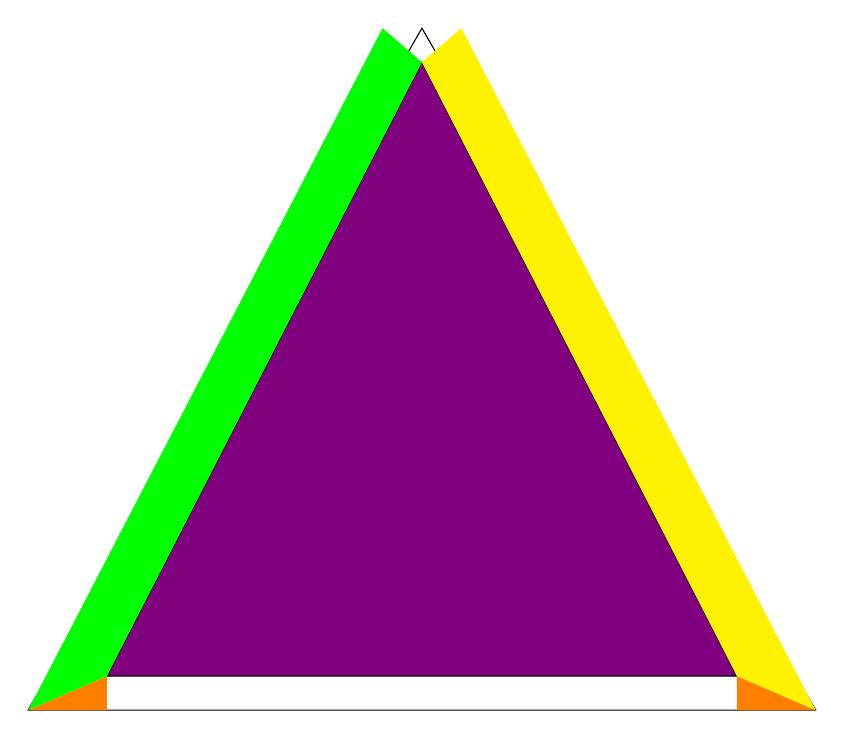
\begin{tikzpicture}
		% Define the length of the sides of the triangles
		\def\sidelength{10}
		
		% Calculate the height of the equilateral triangle
		\pgfmathsetmacro{\triangleheight}{sqrt(3)/2*\sidelength}
		
		% Draw the large outer triangle (white background)
		\draw[fill=white] (0,0) -- (\sidelength,0) -- (0.5*\sidelength, \triangleheight) -- cycle;
		
		% Draw the main central triangle (purple)
		\draw[fill=blue!50!red] (0.1*\sidelength, 0.05*\triangleheight) -- (0.9*\sidelength, 0.05*\triangleheight) -- (0.5*\sidelength, 0.95*\triangleheight) -- cycle;
		
		% Draw the colored segments at each edge
		% Bottom edge segments
		\fill[orange] (0,0) -- (0.1*\sidelength,0) -- (0.1*\sidelength, 0.05*\triangleheight) -- cycle;
		\fill[orange] (\sidelength,0) -- (0.9*\sidelength,0) -- (0.9*\sidelength, 0.05*\triangleheight) -- cycle;
		
		% Left edge segments
		\fill[green] (0,0) -- (0.1*\sidelength, 0.05*\triangleheight) -- (0.5*\sidelength, 0.95*\triangleheight) -- (0.45*\sidelength, \triangleheight) -- cycle;
		
		% Right edge segments
		\fill[yellow] (\sidelength,0) -- (0.9*\sidelength, 0.05*\triangleheight) -- (0.5*\sidelength, 0.95*\triangleheight) -- (0.55*\sidelength, \triangleheight) -- cycle;
		
	\end{tikzpicture}
	\caption{Stylized triangle plot created with TikZ.}
	\label{antennen:tikzparam3eck}
\end{figure}

dasdasd \ref{antennen:tikzparam3eck} dasda